\chapter{Research Context}
\graphicspath{{Chapter2/Figs/}{Chapter2/Figs/}}

This chapter describes the context of the research question and the findings from the current literature. The reader is educated specifically on the limitations of current non-invasive and unidirectional BCIs, the paradigm shift in developing cloud-based and production-ready software versus running software in a research environment, and the implications and hypotheses of web-based approaches to BCIs and 3D applications for VR and AR that relate to the future of software in general in the field of spatial computing.

\section{Limitations of BCIs}
\label{chapter2-limitations-of-bcis}

The capabilities of BCIs are not without limitations. In addition to the physical limitations, mainly in material science for the hardware aspects of BCIs, the author attempts to address a broader issue related to neuropsychology that directly correlates to the software aspects.

\subsection{Decoding brain data}
\label{chapter2-decoding-brain-data}

As outlined in the previous chapter, a holistic view of BCI must take into account the aspect of decoding measured neural data and making it intelligible to computer software. It is important to emphasise that the task of decoding neural data is different from decoding thoughts, which is a critical factor for software. Moreover, decoding neural data and extracting the thoughts behind it so that the software can understand them are disciplines on their own. For example, getting computers to recognise letters written on a photograph is a very different problem from reading the written words in the sentences (i.e. computer vision and natural language processing).

Another part is understanding the sentences and their meaning, as in natural language understanding (NLU). NLU is considered an AI-hard problem, which means that the difficulty of these computational problems is equivalent to solving the central problem of artificial general intelligence (AGI) \citep{demasi_theoretical_2010}, assuming that general human-level intelligence is computational. Understanding less structured data, such as EEG data, is more complicated than understanding structured and human-generated syntax such as written language because it contains more hidden features than a paragraph of text. As a result, the author assumes that understanding brain data might be considered an AI-hard problem.

\subsection{Abstract thoughts}
\label{chapter2-abstract-thoughts}

\begin{figure}[ht]
  \centering
  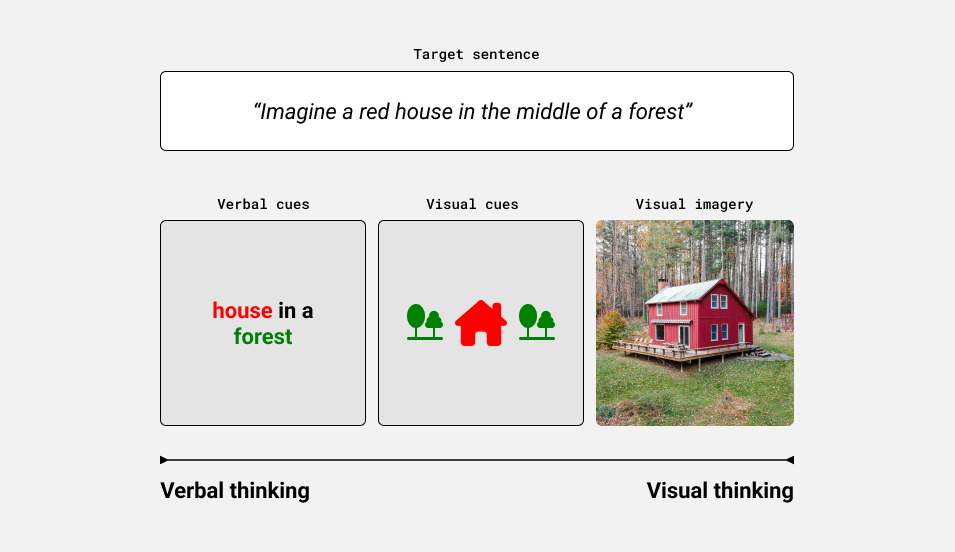
\includegraphics[width=\linewidth]{visual-thinking.png}
  \caption{Difference between verbal and visual thinking using the target sentence of a red house in the middle of a forest (own representation, 2022).}
  \label{fig:visual-thinking}
\end{figure}

Imagine a red house in the middle of a forest. Depending on the individual thought process, one can imagine the house with temporary visual imagery in mind, as in visual thinking, or one can imagine it more verbally, such as conceptually comprehending each word sequentially of what a red house is and that it is located in a forest \citep{amit_asymmetrical_2017}. Additionally, it should also be addressed that different types of thoughts exist at different levels of abstraction and complexity. One can assume that the visual image of a red house in the forest is more abstract and far-fetched than, say, the movement of one's own left arm which has a clear physical counterpart. It gets even more complicated when one imagines concepts that are inconceivable to visualise, such as the idea of a company. A company is only an abstract, collectively agreed upon concept without a physical counterpart and is, therefore, even less straightforward and more complex to decode the meaning of measured brain activity than the other mentioned examples of the red house.

\subsection{Technical limitations}
\label{chapter2-technical-limitations}

\begin{figure}[ht]
  \centering
  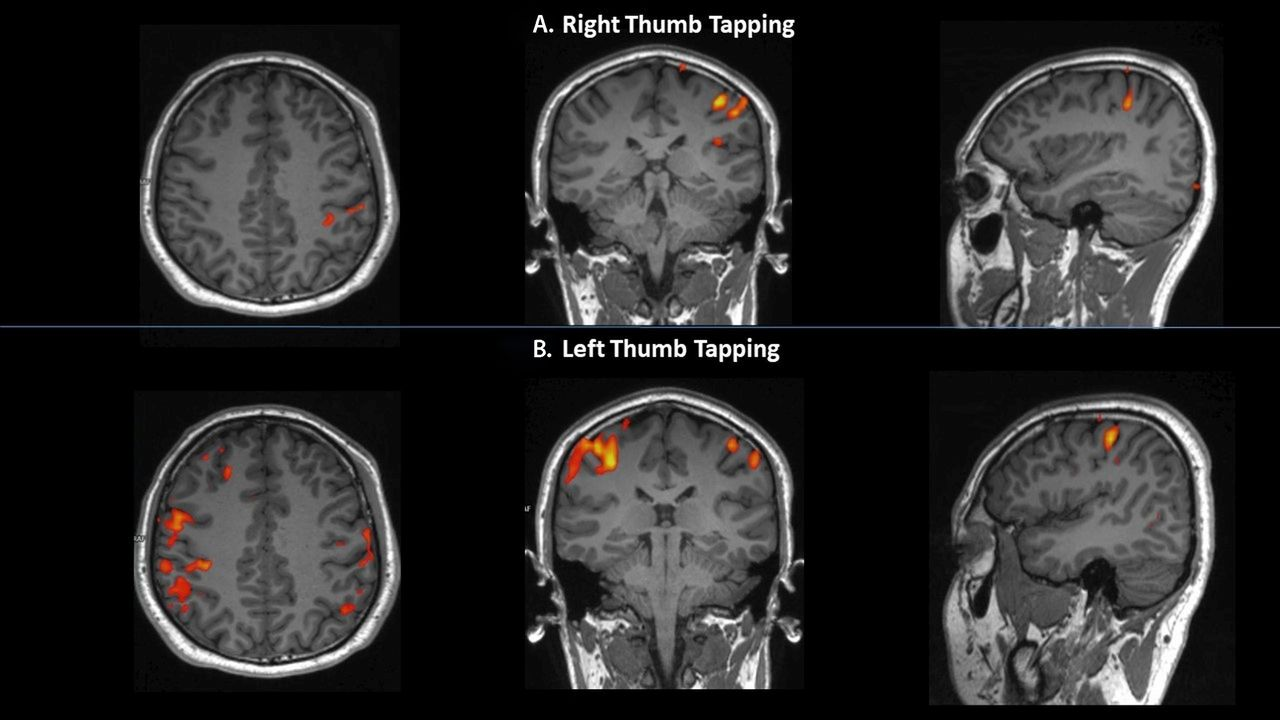
\includegraphics[width=\linewidth]{fmri-scan.jpg}
  \caption{Image of localised activation of neurons during right and left thumb movement using functional magnetic resonance imaging (fMRI) \citep{rashid_bilateral_2018}.}
  \label{fig:fmri-scan}
\end{figure}

Functional tasks of the brain are localised, which means that these signals are generated by local brain areas that can be identified, such as the motor cortex, which has been shown to be responsible for muscle movement as shown on Figure \ref{fig:fmri-scan}. Examining the areas of the brain responsible for activating individual muscle strands can yield a comparable response of muscle stimulation in the brain and thus be measured as output for software to move a prosthesis, for example. However, the more specific, less-functional or abstract the thoughts are, the less the brain areas are spatially visible. To quest to identify, for example, the thought of a red house in a forest in verbal thought, can be classified into three technical problem statements:

\begin{itemize}
  \item To understand abstract thoughts, one would need sufficiently clear data from experiments with a certain level of detail (e.g., at the level of detail related to the firing of individual neurons) as well as temporal precision (an action potential takes about 1 ms to arise, so the precision would need to be in the same range) to perform studies to extract localisations of individual thoughts. Current neuroimaging technology and sensors cannot capture every process in sufficient detail of the entire brain to extract the activity of individual neurons and synapses.
  \item Too much data generated not possible to work with it
  \item Even if we have the technology, it's hard to generate clean brain data that is comparable to previously recorded brain data, because we're all different from each other, we change over time (neuroplasticity) and we are in different states of mind (different sleep, something bothering someone etc.). % TODO Incorporate this paper \citep{hu_model_2021}
        % reproducibility of experiments needed for neuroscience and understanding the brain

\end{itemize}

% TODO Add example from the paper of the CPU
% TODO Add this: https://www.researchgate.net/figure/Machine-learning-model-complexity-and-possible-effects-on-interpretability-model_fig2_346196638

\subsection{Lack of data}
\label{chapter2-lack-of-data}

%  Incorporate this: https://www.nature.com/articles/d41586-022-00767-3

\subsection{Low risk and low impact}
\label{chapter2-low-risk-and-low-impact}

% technical limitations, collected from various neurons, relative high abstraction extracting

% difference between BCI interfacing and just collecting data

% we don't know where to search, we might have a large data set

% Different ways of how a BCI works as of today (talk with Michel), functional and anatomical differences in the brains, some people just work different

% brain states better for non-invasive (state of mind), detailed thoughts

% mobile fmri then might be able to collect detailed thoughts instead of state of mind

% no biggest data set is probably the thing that makes some stuff possible we never have thought about

% still lots of homework to do on the (computational, physiological) neuroscience side

% big inter and intra variability in the brains, brains can be influenced by everything: what u think about, what u ate, what happened, how you slept, what for memories etc.

% mostly hardware needs to be right for bidirectional

% not so reliable and robust, that's why low risk and low impact

% there are chemical processes involved: how much information is even involved in the electricity and not other part?

\section{BCI landscape}
\label{chapter2-research-landscape}

% Current landscape of non-invasive BCIs and their applications (take IDUN's competition overview as a starter point)

\subsection{Real-world BCI applications}
\label{chapter2-real-world-bci-applications}

% Current state of EEG-based games and applications for the normal user (steady state invoked etc.) (talk with Michel and do own research)

% everything is a neural interface, even our own body

% external stimuli, like a sound or light

% personal thoughts: active and passive; make difference of wearable and passive

% "sinnesorgan": motor stuff, visual, auditory, neurofeedback (learn how to control your thoughts, attention training for adhs e.g.) etc.

\subsection{Unobtrusive hardware and software}
\label{chapter2-unobtrusive-hardware-and-software}

% What it takes for a BCI to be mainstream-ready with IDUN as an example (talk with Simon and example of smart glasses)

\subsection{Active and passive BCIs}
\label{chapter2-active-and-passive-bcis}

% Passive brain-computer interfaces and user experience (read paper on passive brain-computer interfaces)

\section{Production-grade software}
\label{chapter2-production-grade-software}

% What production-grade software separates from others
% Use The Twelve Factors as a reference

\subsection{Cloud paradigm-shift}
\label{chapter2-cloud-paradigm-shift}

% Challenges and requirements of going with a cloud, API and SDK (privacy, security, IP, performance, scaling etc.)

\subsection{Web-first BCI architecture}
\label{chapter2-web-first-bci-architecture}

% Examples of BCI data going through web stacks, how to make it work (paper from Stegman)

\subsection{3D applications in the browser}
\label{chapter2-3d-applications-in-the-browser}

% Current state of 3D on the web (WebGPU, pixel streaming, declarative graphics components, WebAssembly (and Rust), etc.)

\subsection{Web-based AR and VR}
\label{chapter2-web-based-ar-and-vr}

% Current state of VR and AR applications (Meta Quest, Snapchat, ARKit, etc.)

\section{N/CI challenges}
\label{chapter2-nci-challenges}

% General challenges of a N/CI

% Akademischer Hintergrund: Vorbilder, Referenzmaterial, Eingrenzung und vertiefte Begründung der Zielformulierung. Grundlagenforschung im Bereich vergleichbarer Medienprodukte. Kenntnis der fachspezifischen Theorien und Techniken. Hier muss umfassende Fach- und Handwerkskenntnis gezeigt werden. Es sollen möglichst viele Informationen verwendet werden, die helfen sollen Entscheidungen für die Erstellung des eigenen Medienprodukts zu treffen und Vorgehensweisen beim Entstehungsprozess des eigenen Medienprodukts zu begründen. Ebenso soll begründet werden, inwiefern die verwendeten Quellen für die Zielsetzung und deren Umsetzung geeignet sind.

\nomenclature[nlu]{NLU}{Natural language understanding}
\nomenclature[agi]{AGI}{Artificial general intelligence}
\nomenclature[fmri]{fMRI}{Functional magnetic resonance imaging}
